\chapter{Łączenie działania deskryptorów}
\label{cha:laczenie}

\section{Wprowadzenie}
Biorąc pod uwagę to, że każdy z elementów wektora traktowany jest przez klasyfikator jako zmienna niezależna od reszty, połączenie wynikowych wektorów dwóch lub więcej metod powinno pozwolić na jeszcze dokładniejsze opisanie danego obiektu. Szczególną korzyść można odnieść w przypadku, gdy łączone ze sobą deskryptory dokonują ekstrakcji cech z oryginalnego obrazu stosując odmienne podejście, dzięki czemu w nowo powstałych wektorach nie ma powielonych redundantnych informacji. Oczywiście kosztem potencjalnego poprawienia skuteczności metody, oprócz konieczności wyliczenia kilku wektorów cech, jest zwiększenie wymiarowości wynikowego wektora cech, co ciągnie za sobą dłuższy czas treningu klasyfikatora i klasyfikacji.

W przebadanych metodach, zarówno HOG jak kowariancja cech, bazują na informacjach dotyczących krawędzi obrazu wejściowego. Odmienne podejście zastosowano w metodzie LBP, która dokonuje ekstrakcji informacji dotyczących tekstury na obrazie. Biorąc pod uwagę powyższe, przebadano zachowanie następujących połączeń deskryptorów: HOG i LBP oraz macierzy kowariancji cech i LBP.

\section{Łączenie deskryptora kowariancji i LBP}

\subsection{Wyniki pierwszej walidacji}

W tabeli \ref{tab:covlbp_first} zestawiono wyniki krzyżowej walidacji pierwszego klasyfikatora wytrenowanego 
próbkami uzyskanymi w wyniku połączenia deskryptorów cech, wykorzystującego macierz kowariancji oraz LBP. Dla porównania zestawiono te wyniki z wynikami uzyskanymi dla pojedynczych deskryptorów.

\begin{center}
    \begin{longtable}{ | p{5cm} | p{3cm} | p{3cm} | p{3cm} |}
    \caption{Wyniki pierwszej walidacji krzyżowej przy użyciu łączonego deskryptora wykorzystującego macierz kowariancji cech i LBP}
    \label{tab:covlbp_first}\\
    \hline
	Metoda & Kowariancja & LBP & Połączenie \\ \hline
    Długość wektora cech & 832 & 4096 & 4928 \\ \hline
    Liczba pozytywnych detekcji w pozytywnym zbiorze testowym & 593 & 531 & 601 \\ \hline
    Liczba negatywnych detekcji w pozytywnym zbiorze testowym & 33 & 95 & 25 \\ \hline
    Celność metody w pozytywnym zbiorze testowym & \textbf{94,73\%} & \textbf{84,82\%} & \textbf{96,01\%} \\ \hline
    Liczba pozytywnych detekcji w negatywnych zbiorze testowym & 30 & 20 & 21 \\ \hline
    Liczba negatywnych detekcji w negatywnym zbiorze testowym & 876 & 886 & 885 \\ \hline
    Celność metody w negatywnym zbiorze testowym & \textbf{96,69\%} & \textbf{97,79\%} & \textbf{97,68\%} \\ \hline
    
    \end{longtable}
\end{center}


\subsection{Wyniki drugiej walidacji}
W tabeli \ref{tab:covlbp_second} zestawiono wyniki krzyżowej walidacji drugiego klasyfikatora po dotrenowaniu pierwszego klasyfikatora fałszywymi pozytywnymi detekcjami, wykrytymi w zbiorze testowym. W celu zminimalizowania efektu "przetrenowania" klasyfikatora wzięto pod uwagę 25\% fałszywie pozytywnych detekcji wygenerowanych na zbiorze testowym. Dla porównania zestawiono te wyniki z wynikami uzyskanymi dla pojedynczych deskryptorów.

\begin{center}
    \begin{longtable}{ | p{5cm} | p{3cm} | p{3cm} | p{3cm} |}
    \caption{Wyniki drugiej walidacji krzyżowej przy użyciu łączonego deskryptora wykorzystującego macierz kowariancji cech i LBP}
    \label{tab:covlbp_second}\\
    \hline
	Metoda & Kowariancja & LBP & Połączenie \\ \hline
    Długość wektora cech & 832 & 4096 & 4928 \\ \hline
    Liczba pozytywnych detekcji w pozytywnym zbiorze testowym & 502 & 512 & 584 \\ \hline
    Liczba negatywnych detekcji w pozytywnym zbiorze testowym & 124 & 134 & 40 \\ \hline
    Celność metody w pozytywnym zbiorze testowym & \textbf{80,20\%} & \textbf{81,79\%} & \textbf{93,29\%} \\ \hline
    Liczba pozytywnych detekcji w negatywnych zbiorze testowym & 19 & 30 & 17 \\ \hline
    Liczba negatywnych detekcji w negatywnym zbiorze testowym & 887 & 876 & 889 \\ \hline
    Celność metody w negatywnym zbiorze testowym & \textbf{97,90\%} & \textbf{96,69\%} & \textbf{98,12\%} \\ \hline
    \end{longtable}
\end{center}


\subsection{Rozkłady błędów detekcji}

Wykres rozkładu błędu detekcji przy połączeniu deskryptorów HOG i LBP zaprezentowany został na rysunku \ref{fig:covlbp_det}. Na podstawie wykresu można zauważyć, że połączenie metod wyraźnie poprawia skuteczność działania metody dla takiego samego rzędu fałszywie pozytywnych detekcji na obrazie. 

\begin{figure}[htb]
\centering
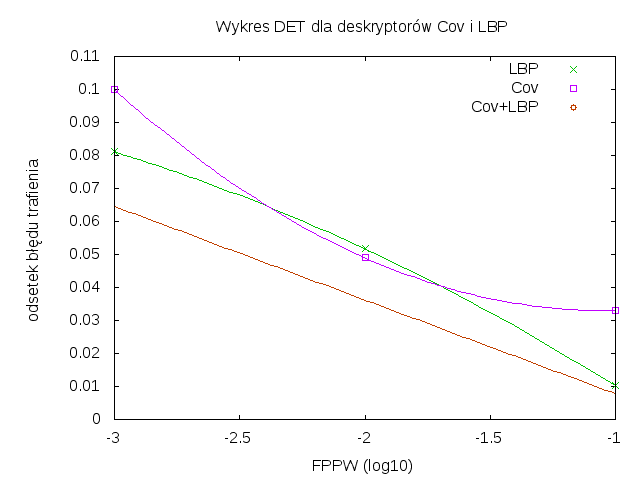
\includegraphics[width=0.9\textwidth]{covlbp_det.png}
\caption{Rozkład błędu detekcji dla połączenia metody LBP i kowariancji cech}
\label{fig:covlbp_det}
\end{figure}

\subsection{Analiza złożoności poszczególnych kroków metody}

W poniższej tabeli zestawiono czasy wykonywania poszczególnych kroków metodologii na konfiguracji testowej.
Dla porównania zestawiono te wyniki z wynikami uzyskanymi dla pojedynczych deskryptorów.

\begin{center}
    \begin{longtable}{ | p{5cm} | p{3cm} | p{3cm} | p{3cm} |}
    \hline
	Metoda & Kowariancja & LBP & Połączenie \\ \hline
    Ekstrakcja cech pozytywnych / próbka & 4,33 ms & 11,08 ms & 14,72 ms \\ \hline
    Ekstrakcja cech negatywnych / próbka & 3,54 ms & 10,19 ms & 13,86 ms\\ \hline
    Pierwszy trening klasyfikatora & 10,75 s & 27,67 s & 57,67 s \\ \hline
    Generacja fałszywie pozytywnych okien & 296,06 s & 657 s & 884,73 s \\ \hline
    Drugi trening klasyfikatora & 14,41 s & 31,62 s & 68,62 s \\ \hline
    Analiza rozkładu błędu detekcji w zbiorze testowym & 3172 s & 4914 s & 5200 s \\ \hline
    \caption{Czas wykonywania poszczególnych etapów badania przy użyciu łączonego deskryptora wykorzystującego macierz kowariancji cech i LBP} \\
    \end{longtable}
\end{center}

\subsection{Podsumowanie}

Nowo utworzony deskryptor można, pod względem jakościowym, ocenić znacznie lepiej niż jego pojedyncze składowe, używane do detekcji osobno. Potwierdza to zarówno rozkład DET porównany z~rozkładami dla składowych jak i wyniki krzyżowych walidacji, w szczególności po dotrenowaniu klasyfikatora. Odbywa się to jednak zwiększonym kosztem złożoności użycia nowej metody. Wynika to bezpośrednio z faktu, że klasyfikator operuje na znacznie większych wektorach cech, które powstają z połączenia dwóch.


\section{Łączenie deskryptora HOG i LBP}

\subsection{Wyniki pierwszej walidacji}

W poniższej tabeli zestawiono wyniki krzyżowej walidacji pierwszego klasyfikatora wytrenowanego 
próbkami uzyskanymi w wyniku połączenia deskryptorów cech, wykorzystującego deskryptory HOG oraz LBP. Dla porównania zestawiono te wyniki z wynikami uzyskanymi dla pojedynczych deskryptorów.

\begin{center}
    \begin{longtable}{ | p{5cm} | p{3cm} | p{3cm} | p{3cm} |}
    \hline
	Metoda & HOG & LBP & Połączenie \\ \hline
    Długość wektora cech & 7308 & 4096 & 11404 \\ \hline
    Liczba pozytywnych detekcji w pozytywnym zbiorze testowym & 575 & 531 & 585 \\ \hline
    Liczba negatywnych detekcji w pozytywnym zbiorze testowym & 57 & 95 & 41 \\ \hline
    Celność metody w pozytywnym zbiorze testowym & \textbf{91,85\%} & \textbf{84,82\%} & \textbf{93,45\%} \\ \hline
    Liczba pozytywnych detekcji w negatywnych zbiorze testowym & 31 & 20 & 21 \\ \hline
    Liczba negatywnych detekcji w negatywnym zbiorze testowym & 875 & 886 & 885 \\ \hline
    Celność metody w negatywnym zbiorze testowym & \textbf{96,58\%} & \textbf{97,79\%} & \textbf{97,68\%} \\ \hline
    \caption{Wyniki pierwszej walidacji krzyżowej przy użyciu łączonego deskryptora wykorzystującego deskryptory HOG i LBP} \\
    \end{longtable}
\end{center}


\subsection{Wyniki drugiej walidacji}
W poniższej tabeli zestawiono wyniki krzyżowej walidacji drugiego klasyfikatora po dotrenowaniu pierwszego klasyfikatora fałszywymi pozytywnymi detekcjami, wykrytymi w zbiorze testowym. W celu zminimalizowania efektu "przetrenowania" klasyfikatora wzięto pod uwagę 25\% fałszywie pozytywnych detekcji wygenerowanych na zbiorze testowym. Dla porównania zestawiono te wyniki z wynikami uzyskanymi dla pojedynczych deskryptorów.

\begin{center}
    \begin{longtable}{ | p{5cm} | p{3cm} | p{3cm} | p{3cm} |}
    \hline
	Metoda & HOG & LBP & Połączenie \\ \hline
    Długość wektora cech & 7308 & 4096 & 11404 \\ \hline
    Liczba pozytywnych detekcji w pozytywnym zbiorze testowym & 531 & 512 & 564 \\ \hline
    Liczba negatywnych detekcji w pozytywnym zbiorze testowym & 95 & 134 & 60 \\ \hline
    Celność metody w pozytywnym zbiorze testowym & \textbf{84,82\%} & \textbf{81,79\%} & \textbf{90,10\%} \\ \hline
    Liczba pozytywnych detekcji w negatywnych zbiorze testowym & 32 & 30 & 13 \\ \hline
    Liczba negatywnych detekcji w negatywnym zbiorze testowym & 874 & 876 & 893 \\ \hline
    Celność metody w negatywnym zbiorze testowym & \textbf{96,47\%} & \textbf{96,69\%} & \textbf{98,57\%} \\ \hline
    \caption{Wyniki drugiej walidacji krzyżowej przy użyciu łączonego deskryptora wykorzystującego deskryptory HOG i LBP} \\
    \end{longtable}
\end{center}


\subsection{Rozkłady błędów detekcji}

Wykres rozkładu błędu detekcji przy połączeniu deskryptorów HOG i LBP zaprezentowany został na rysunku \ref{fig:hoglbp_det}. Na podstawie wykresu można zauważyć, że połączenie tych metod nie poprawia działania klasyfikatora, a w kontekście zbioru testowego i metodologii, na którym został badany nawet nieco pogarsza.

\begin{figure}[htb]
\centering
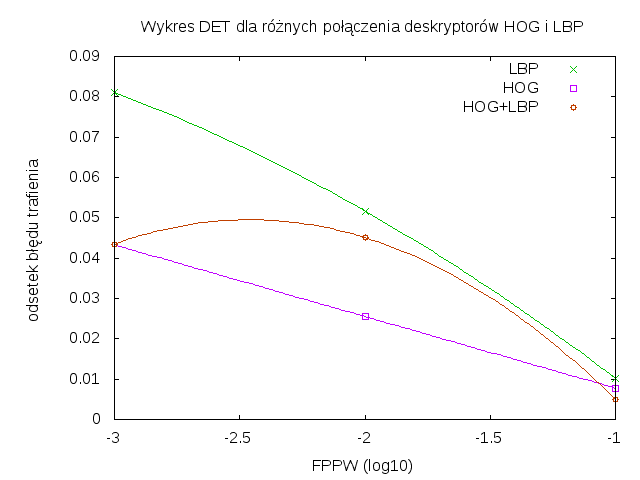
\includegraphics[width=0.9\textwidth]{hoglbp_det.png}
\caption{Rozkład błędu detekcji dla połączenia metody LBP iHOG}
\label{fig:hoglbp_det}
\end{figure}

\subsection{Analiza złożoności poszczególnych kroków metody}

W poniższej tabeli zestawiono czasy wykonywania poszczególnych kroków metodologii na konfiguracji testowej.
Dla porównania zestawiono te wyniki z wynikami uzyskanymi dla pojedynczych deskryptorów.

\begin{center}
    \begin{longtable}{ | p{5cm} | p{3cm} | p{3cm} | p{3cm} |}
    \hline
	Metoda & HOG & LBP & Połączenie \\ \hline
    Ekstrakcja cech pozytywnych / próbka & 6,23 ms & 11,08 ms & 15,24 ms \\ \hline
    Ekstrakcja cech negatywnych / próbka & 5,27 ms & 10,19 ms & 14,05 ms\\ \hline
    Pierwszy trening klasyfikatora & 33,69 s & 27,67 s & 69,89 s \\ \hline
    Generacja fałszywie pozytywnych okien & 590,40 s & 657 s & 987,32 s \\ \hline
    Drugi trening klasyfikatora & 40,62 s & 31,62 & 82,39 s \\ \hline
    Analiza rozkładu błędu detekcji w zbiorze testowym & 1938 s & 4914 s & 5730 s \\ \hline
    \caption{Czas wykonywania poszczególnych etapów badania przy użyciu łączonego deskryptora wykorzystującego macierz kowariancji cech i LBP} \\
    \end{longtable}
\end{center}

\subsection{Podsumowanie}
Biorąc pod uwagę wyniki walidacji krzyżowej, z której można wywnioskować nieznaczną poprawę działania deskryptora HOG, a także wykres rozkładu błędu detekcji, który sugeruje negatywny wpływ połączenia, można dojść do wniosku, że w kontekście detekcji sylwetek ludzkich deskryptor LBP w~słabym stopniu uzupełnia metodę HOG.